% -- Document configuration
\documentclass{article}

% -- Input and language settings
% \usepackage[utf8]{inputenc}
\usepackage[spanish]{babel}
\decimalpoint                             % From babel package to use points instead of commas in decimals

% -- Page and line settings
\usepackage{geometry}
\geometry{letterpaper, 
    % margin=2cm, 
    left=3cm, right=3cm,
    top=1.2cm, bottom=1.2cm,
    includefoot, 
    includehead}
\renewcommand{\baselinestretch}{1.2}

% -- Required packages
\usepackage{xcolor}
\usepackage[many]{tcolorbox}
\usepackage{mathtools,amsfonts,amsmath}     % Loads amsmath if not already loaded
\allowdisplaybreaks                         % To allow page breaks if equations are too long
\usepackage[parfill]{parskip}               % No indent and separation lines for paragraphs
\usepackage{cancel}                         % To cancel math terms
\usepackage[shortlabels]{enumitem}          % To handle enumerations
\usepackage{tikz}
\usetikzlibrary{automata, arrows.meta, positioning}
\usepackage[mode=buildnew]{standalone}      % To import figures in standalone files
\usepackage[hidelinks]{hyperref}
\usepackage[spanish]{cleveref}              % To use autocompleted reference labels, language must be change as in babel package
\usepackage{caption}                        % Caption and subcaption to allow subfigures
\usepackage{subcaption}
\usepackage{float}                          % To specify the location of figures
\usepackage{multicol}                       % To use multicolumns
\usepackage[bottom]{footmisc}               % To locate footnotes at the bottom

% -- Title and heading settings
\usepackage{titling}
\usepackage{fancyhdr}
\pagestyle{fancy}

% -- Code and code formatting
\usepackage{minted}                         % To insert code
\usemintedstyle[julia]{gruvbox-light}       % Code theme and language
\definecolor{bg}{rgb}{0.98, 0.97, 0.88}     % Code block background

\usepackage{fontspec}                       % To allow the use of monospace fonts
\setmonofont{JuliaMono}[Path=./codefonts/, Extension=.ttf, UprightFont=*-Regular, ItalicFont=*-RegularItalic, Scale=0.75]

\usepackage{fancyvrb}                       % To change line number font
\renewcommand{\theFancyVerbLine}{\textcolor{gray}{\footnotesize\texttt{\arabic{FancyVerbLine}}}}

\definecolor{light-gray}{gray}{0.95}        % Color, box and style to show small code thingys inside normal text
\newcommand{\code}[1]{\colorbox{light-gray}{\texttt{#1}}}

% -- Bilbiography preferences
\usepackage[square,numbers]{natbib}
\bibliographystyle{unsrt}

% -- Footnotes without numbering
\newcommand\nnfootnote[1]{%
  \begin{NoHyper}
  \renewcommand\thefootnote{}\footnote{#1}%
  \addtocounter{footnote}{-1}%
  \end{NoHyper}
}

% -- Theorems
\newtheorem{theorem}{Theorem}

\lhead{\theinstitution\ -- \thedepartment}
\chead{}
\rhead{Programación para la IA\ -- \thetitle}
\lfoot{}
\cfoot{\thepage}
\rfoot{}

% -- Problem solution
\newenvironment{solution}
{\begin{quote}
\textbf{Solución:}\medskip

}
{

\hfill\rule{0.5\textwidth}{0.5pt}
\end{quote}}

% -- Equation result
\newcommand{\result}[1]
{
\tcbhighmath[colframe=white, colback=gray!15, sharp corners]
{#1}
}

% -- Function definitions
\newcommand{\dprod}[2]{{#1} \cdot {#2}}
\newcommand{\txtgray}[1]{\textcolor{gray}{#1}}

% -- Author information
\title{Actividad 5}
\author{Leonardo Flores Torres}
\newcommand\theinstitution{Universidad Veracruzana}
\newcommand\thedepartment{Inteligencia Artificial}
\newcommand\thecourse{Programación para la Inteligencia Artificial}

% -- Paths
% \newcommand\codelists{../programs/lists.rkt}

% Remove red color boxes of "syntax errors" in minted
\AtBeginEnvironment{minted}{%
  \renewcommand{\fcolorbox}[4][]{#4}}

% -- Document
\begin{document}

\thispagestyle{empty}

%Title
\begin{center}
\textsc{\theinstitution}\\[2mm]

\thedepartment

\rule{0.6\textwidth}{0.5pt}\\[2mm]

\thecourse \\[4mm]

{\Large \textbf{\thetitle}}\\[2mm]

\theauthor \\[2mm]

{\small \today}
\end{center}
\medskip

% -- 
\vspace{1cm}

\textbf{Resolución del problema del viajero utilizando recocido simulado.}

A partir de las coordenadas de las capitales de México, en cada ejecución del algoritmo:
\begin{enumerate}
    \item Dar el valor del número $N$ de ciudades que se utilizaran.
    \item Hacer una selección aleatoria de $N'$ ciudades.
    \item Resolver el problema del viajero para ese conjunto de ciudades empleando el algoritmo de recocido simulado.
    \item Para un número $N'$ de ciudades menor que 10 compare la solución $d_s$ obtenida por recocido simulado con la solución $d^{\star}$ que se genera al computar todas las posibilidades $N'!$ mediante fuerza bruta. La comparación debe realizarse en términos del error en la distancia, $E = |d^{\star} - d_s|$.
    \item Probar con al menos 3 valores distintos de $N$, y donde uno de esos valores sea la totalidad de las ciudades capitales de México.
    \item Mostrar de manera gráfica la solución final obtenida en cada caso.
\end{enumerate}

Este problema, \textit{the travelling salesman problem}, es uno de encontrar la ruta más óptima ¿Pero óptima en qué sentido? La proposición inicial del problema fue el de encontrar la ruta que minimize la distancia al recorrer un conjunto de puntos de interés, aunque podría extenderse este concepto a encontrar la ruta que minimize el tiempo al recorres estos puntos, o el costo monetario para completar la ruta. Este problema es, en principio, un problema de minimizar una función y la manera de hacerlo es haciendo alusión a un sistema físico.

Primero se podría pensar, y con toda razón, que es un problema de encontrar la combinación del orden en que se visitan estos puntos de interés la cual dé como resultado la distancia más corta de todo el recorrido. Este razonamiento tiene sentido teóricamente pero hay un problema con ello, al aumentar el número $N$ de puntos de interés a visitar el número de combinaciones crece como $N!$. Si en México se quisieran visitar 5 ciudades entonces se tendrían que obtener todas las permutaciones posibles. El número total de permutaciones es igual a
\begin{equation*}
    _{n}{P}_{r} = \frac{n!}{(n - k)!} ,
\end{equation*}
donde $n$ es el tamaño del conjunto, en este caso la cantitad total de puntos de interés, y $k$ es la el tamaño del subconjunto, que corresponde a la cantidad de puntos de interés que sí se van a visitar del total. Si se visitan todos los puntos de interés, entonces $n = k$ y obtenemos que la cantitad total de permutaciones es igual a $_{n}P_{r} = n!$. Si nuestro conjunto es de 5 ciudades, y se visitarán las 5, entonces el total de permutaciones es 120. Si se tienen 10 ciudades y se visitaran todas, entonces el total de permutaciones aumenta a 3628800. Y si fuesen 15, las permutaciones incrementarian a un ridículo total de 1307674368000 ¿Con tantas maneras distintas de realizar el recorrido cómo se puede encontrar la mejor? El problema parece simple de resolver, sí, cuando no se consideran tantos puntos de interés. El trabajo presente apunta a encontrar una solución a esta incógnita tomando a los puntos de interés como las capitales de México siendo un total de 32.

Antes de continuar quisiera mencionar que no fui capaz de realizar el cómputo mediante fuerza bruta considerando el total de capitales lo cuál era de esperarse, ya que computar todas las permutaciones requiere memoria y la librería en \code{julia} disponible para el cómputo de permutaciones depende de la función \code{factorial} la cual tiene una restricción, no puede ser usada para valores mayores a 20. Por lo que \code{factorial(21)} ya no computa.

\begin{figure}[ht!]
    \centering
    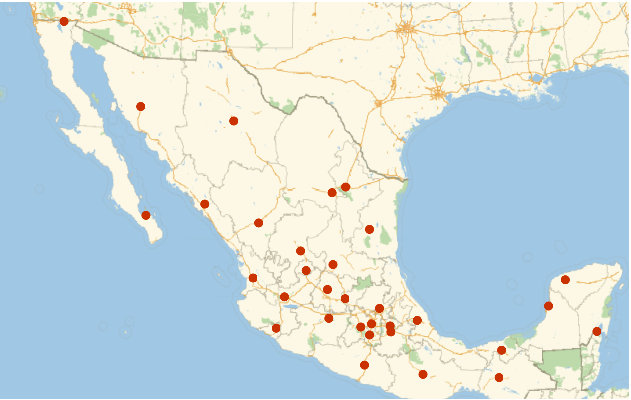
\includegraphics[scale=0.8]{../figures/capital_locations.pdf}
    \caption{Ubicación de las capitales de México.}
    \label{fig:capitales_mexico}
\end{figure}

Las capitales de México se pueden ver ubicadas en la \cref{fig:capitales_mexico} con circulos de color rojo, siendo un total de 32. Las coordenadas fueron obtenidas usando GoogleMaps buscando cada ciudad y tomando sus coordenasas aproximadamente en sus centros. Se implementó una función para guardar la inforación de las capitales, \code{available\_cities} y usarla posteriormente cuando se necesite hacer una selección aleatoria de las mismas.

Comenzaremos tomando 5 ciudades de manera aleatoria, se mostrarán los nombres de las ciudades seleccionadas (en el orden en que se visitarán) junto con sus latitudes y longitudes correspondientes, como se muestra a continuación:
\begin{minted}[
    frame=none,
    autogobble,
    obeytabs=false,
    breaklines,
    tabsize=4,
    linenos=true,
    baselinestretch=1,
    firstnumber=last,
    bgcolor=bg!70,
    mathescape,
    numberblanklines=false
    ]{julia}
    # Seleccion aleatoria de ciudades
    julia> sample_cities = ts.sample_cities(5);

    # Mostrar ciudades seleccionadas
    julia> map(x -> x.name, sample_cities)
    5-element Vector{String}:
    "oaxaca"
    "saltillo"
    "zacatecas"
    "queretaro"
    "tlaxcala"

    # Mostrar coordenadas de ciudades seleccionadas
    julia> map(x -> (x.lat, x.lon), sample_cities)
    5-element Vector{Tuple{Float64, Float64}}:
    (17.062183511066106, -96.72572385123796)
    (25.425170167352245, -101.00211644466016)
    (22.772858479171045, -102.57341087527752)
    (20.592088731107133, -100.3918227421049)
    (19.314544474512967, -98.23851540921879)
\end{minted}

El mapeo muestra el nombre de las ciudades en el orden en el que se van a visitar, se comienza en Oaxaca y se termina en Tlaxcala. Aunque este es un viaje redondo, esto significa que después de haber llegado Tlaxcala se debe regresar a Oaxaca nuevamente. En la \cref{fig:trip_cities_05_init} se puede observar el recorrido inicial de esta configuración, 
\begin{figure}[ht!]
    \centering
    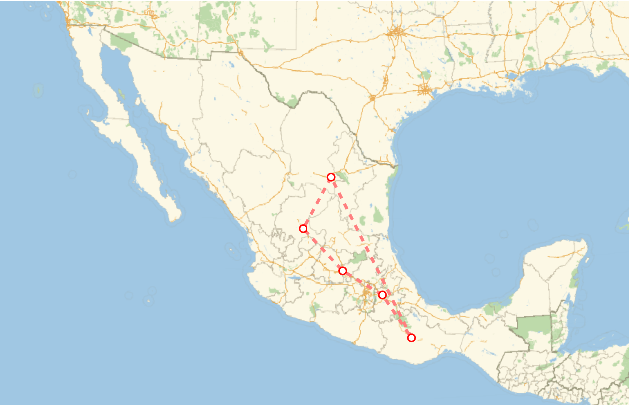
\includegraphics[scale=0.8]{../figures/trip_cities_05_init.pdf}
    \caption{Ruta inicial para cinco capitales comenzando en Oaxaca.}
    \label{fig:trip_cities_05_init}
\end{figure}

El recorrido mostrado en \cref{fig:trip_cities_05_init} es el realizado si se hiciera caso a la selección aleatoria, pero no se desea eso. Primero se calcularán las permutaciones de la selección aleatoria de capitales guardada en \code{sample\_cities}:
\begin{minted}[
    frame=none,
    autogobble,
    obeytabs=false,
    breaklines,
    tabsize=4,
    linenos=true,
    baselinestretch=1,
    firstnumber=last,
    bgcolor=bg!70,
    mathescape,
    numberblanklines=false
    ]{julia}
    # Computando las permutaciones
    julia> path_permutations = ts.brute_force(sample_cities, "geo");

    # Calculando la distancia de cada ruta
    julia> path_permutations_dist = ts.total_distance.(path_permutations, "geo");
\end{minted}

Teniendo las permutaciones se buscará la ruta con la distancia mínima, y también alguna otra ruta cuya distancia sea igual a la mínima como se muestra a continuación:
\begin{minted}[
    frame=none,
    autogobble,
    obeytabs=false,
    breaklines,
    tabsize=4,
    linenos=true,
    baselinestretch=1,
    firstnumber=last,
    bgcolor=bg!70,
    mathescape,
    numberblanklines=false
    ]{julia}
    # Camino de distancia minima
    julia> min_path = path_permutations[argmin(path_permutations_dist)]

    # Distancia minima
    julia> min_dist = minimum(path_permutations_dist)
    2250.1837692021245

    # Buscando los indices del camino o caminos mas cortos cuya distancia sea igual a la minima encontrada
    julia> optimal_indexes = findall(x -> x == min_dist, path_permutations_dist)
    10-element Vector{Int64}:
    15
    19
    33
    44
    59
    62
    77
    88
    102
    106

    # Encontrando las rutas que coinciden con la distancia minima
    julia> map.(x -> x.name, path_permutations[optimal_indexes])
    10-element Vector{Vector{String}}:
    ["oaxaca", "queretaro", "zacatecas", "saltillo", "tlaxcala"]
    ["oaxaca", "tlaxcala", "saltillo", "zacatecas", "queretaro"]
    ["saltillo", "zacatecas", "queretaro", "oaxaca", "tlaxcala"]
    ["saltillo", "tlaxcala", "oaxaca", "queretaro", "zacatecas"]
    ["zacatecas", "saltillo", "tlaxcala", "oaxaca", "queretaro"]
    ["zacatecas", "queretaro", "oaxaca", "tlaxcala", "saltillo"]
    ["queretaro", "oaxaca", "tlaxcala", "saltillo", "zacatecas"]
    ["queretaro", "zacatecas", "saltillo", "tlaxcala", "oaxaca"]
    ["tlaxcala", "oaxaca", "queretaro", "zacatecas", "saltillo"]
    ["tlaxcala", "saltillo", "zacatecas", "queretaro", "oaxaca"]
\end{minted}

De esta manera nos hemos asegurado de encontrar todas las ocurrencias donde las distancias de los caminos son iguales al mínimo encontrado. Si no se hubiése hecho así y solamente se hubiera aplicado la función \code{minimum} sí se que habría detectado un mínimo, pero solamente uno. A pesar de que la primera capital en el muestreo aleatorio de capitales fue Oaxaca esto no restringe aque se deba partir de ahí, y también debe recordarse que todas las rutas mostradas con el mismo resultado son rutas de viaje redondo.
\begin{figure}[ht!]
    \centering
    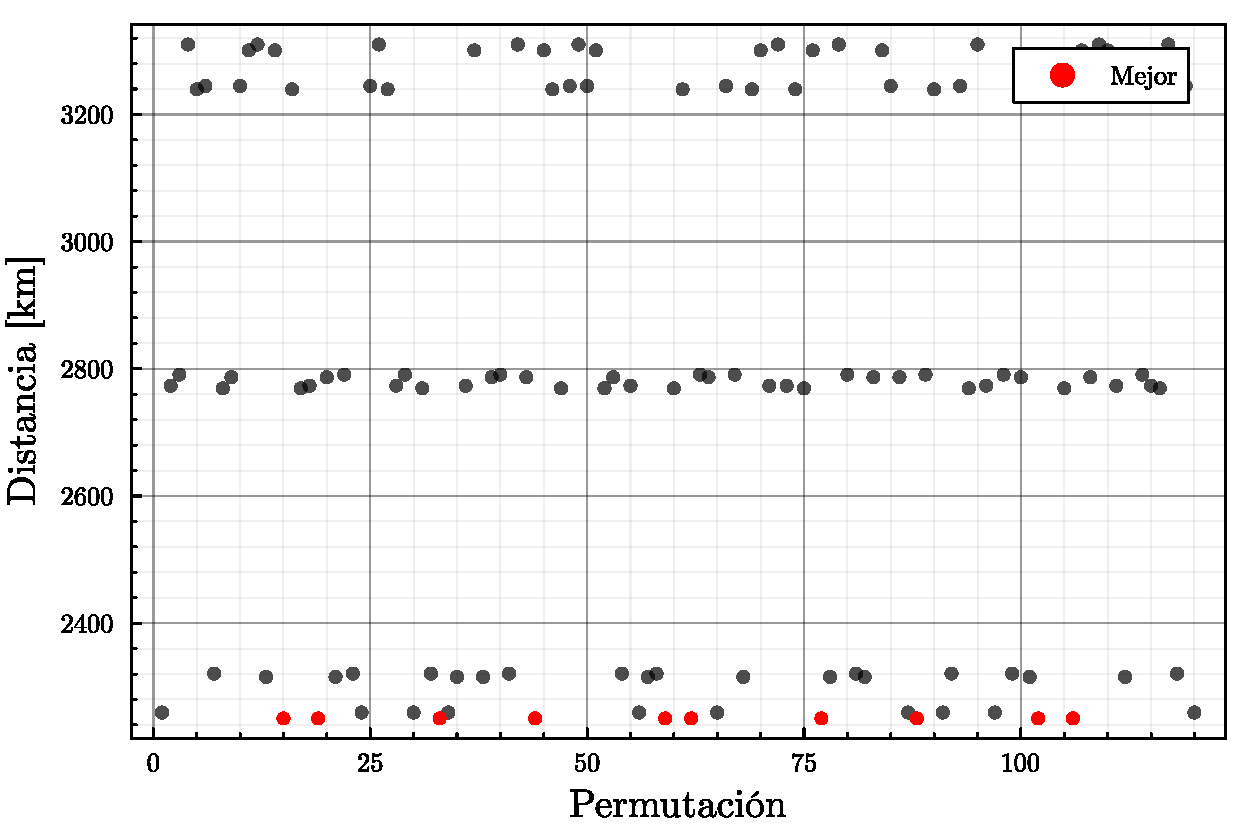
\includegraphics[scale=0.5]{../figures/distances_cities_05_bruteforce.pdf}
    \caption{XXX}
    \label{fig:bruteforce_distances_cities_05}
\end{figure}

De la \cref{fig:bruteforce_distances_cities_05} se puede observar en marcadores rojos aquellas permutaciones con la misma distancia mínima, mienstras que los de color grisáseo son rutas menos óptimas. En realidad se podría elegir cualquier ruta de las marcadas en rojo pero para motivos de este trabajo vamos a trabajar con la guardada en \code{min\_path}. El recorrido de esta ruta se puede observar en XXX,
\begin{figure}[ht]
    \centering
    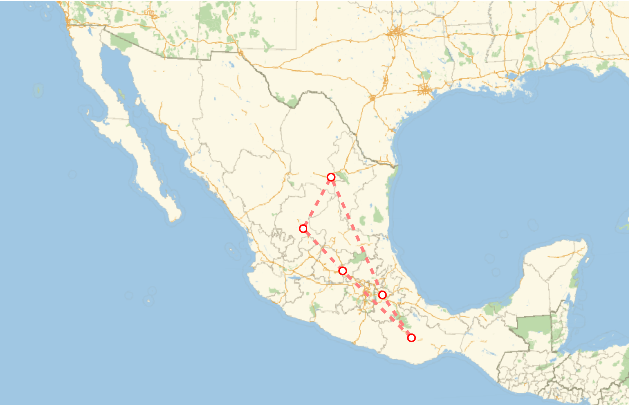
\includegraphics[scale=0.8]{../figures/trip_cities_05_bruteforce.pdf}
    \caption{XXX}
    \label{fig:bruteforce_path_cities_05}
\end{figure}

\clearpage
\section*{Apéndice}
\inputminted[
    frame=none,
    autogobble,
    obeytabs=false,
    breaklines,
    tabsize=4,
    linenos=true,
    baselinestretch=1,
    firstnumber=1,
    bgcolor=bg!70,]{julia}{\codepath}

\nocite{*}    % to call all references even if they are not cited in the text
\bibliography{references.bib}

\end{document}

% \begin{minted}[
%     frame=none,
%     autogobble,
%     obeytabs=false,
%     breaklines,
%     tabsize=4,
%     linenos=true,
%     baselinestretch=1,
%     firstnumber=last,
%     bgcolor=bg!70,
%     mathescape,
%     numberblanklines=false
%     ]{julia}
%     # empty comment
% \end{minted}

